\documentclass{article}
\usepackage{graphicx}
\usepackage{caption}
\usepackage{subcaption}
\usepackage[a4paper, margin=1in]{geometry}
\usepackage{booktabs} % For professional looking tables

\title{Simulation Results of Quadrotor Tracking}
\author{Your Name}
\date{\today}

\begin{document}

\maketitle

\section{Introduction}
This document presents the simulation results for a quadrotor equipped with a gimbal, tasked with tracking a fixed-wing aircraft. The performance of the system is evaluated under two distinct trajectory scenarios: a circular loop and a straight level flight. The simulation models for both the fixed-wing aircraft and the quadrotor are implemented in MATLAB.

\section{System Parameters}
The parameters for the fixed-wing aircraft and the quadrotor are detailed in the tables below.

\begin{table}[h!]
\centering
\caption{Fixed-Wing Aircraft Parameters}
\label{tab:fw_params}
\begin{tabular}{@{}lll@{}}
\toprule
Parameter & Value & Unit \\ \midrule
Mass ($m$) & 13.5 & kg \\
Inertia ($J$) & diag(0.8244, 1.135, 1.759) & kg$\cdot$m$^2$ \\
Wing Area ($S$) & 0.55 & m$^2$ \\
Wingspan ($b$) & 2.8956 & m \\
Mean Chord ($c$) & 0.18994 & m \\
Air Density ($\rho$) & 1.225 & kg/m$^3$ \\
\bottomrule
\end{tabular}
\end{table}

\begin{table}[h!]
\centering
\caption{Quadrotor Parameters}
\label{tab:quad_params}
\begin{tabular}{@{}lll@{}}
\toprule
Parameter & Value & Unit \\ \midrule
Mass ($m$) & 0.468 & kg \\
Inertia ($I_x$) & 0.0023 & kg$\cdot$m$^2$ \\
Inertia ($I_y$) & 0.0023 & kg$\cdot$m$^2$ \\
Inertia ($I_z$) & 0.0046 & kg$\cdot$m$^2$ \\
Gravity ($g$) & 9.81 & m/s$^2$ \\
Arm Length ($l$) & 0.225 & m \\
\bottomrule
\end{tabular}
\end{table}

\section{Simulation Results}

\subsection{Trajectory 1: Level Flight}
For the level flight trajectory, a constant elevator input of -0.05 rad is applied to counteract gravity and maintain a steady flight path. The results demonstrate that the drone accurately follows the reference position of the fixed-wing plane. The gimbal quickly compensates for the oscillations in the drone as it pitches to match the fixed-wing's speed and dynamics. As shown in the figures, the drone perfectly follows the trajectory.

\begin{figure}[h!]
    \centering
    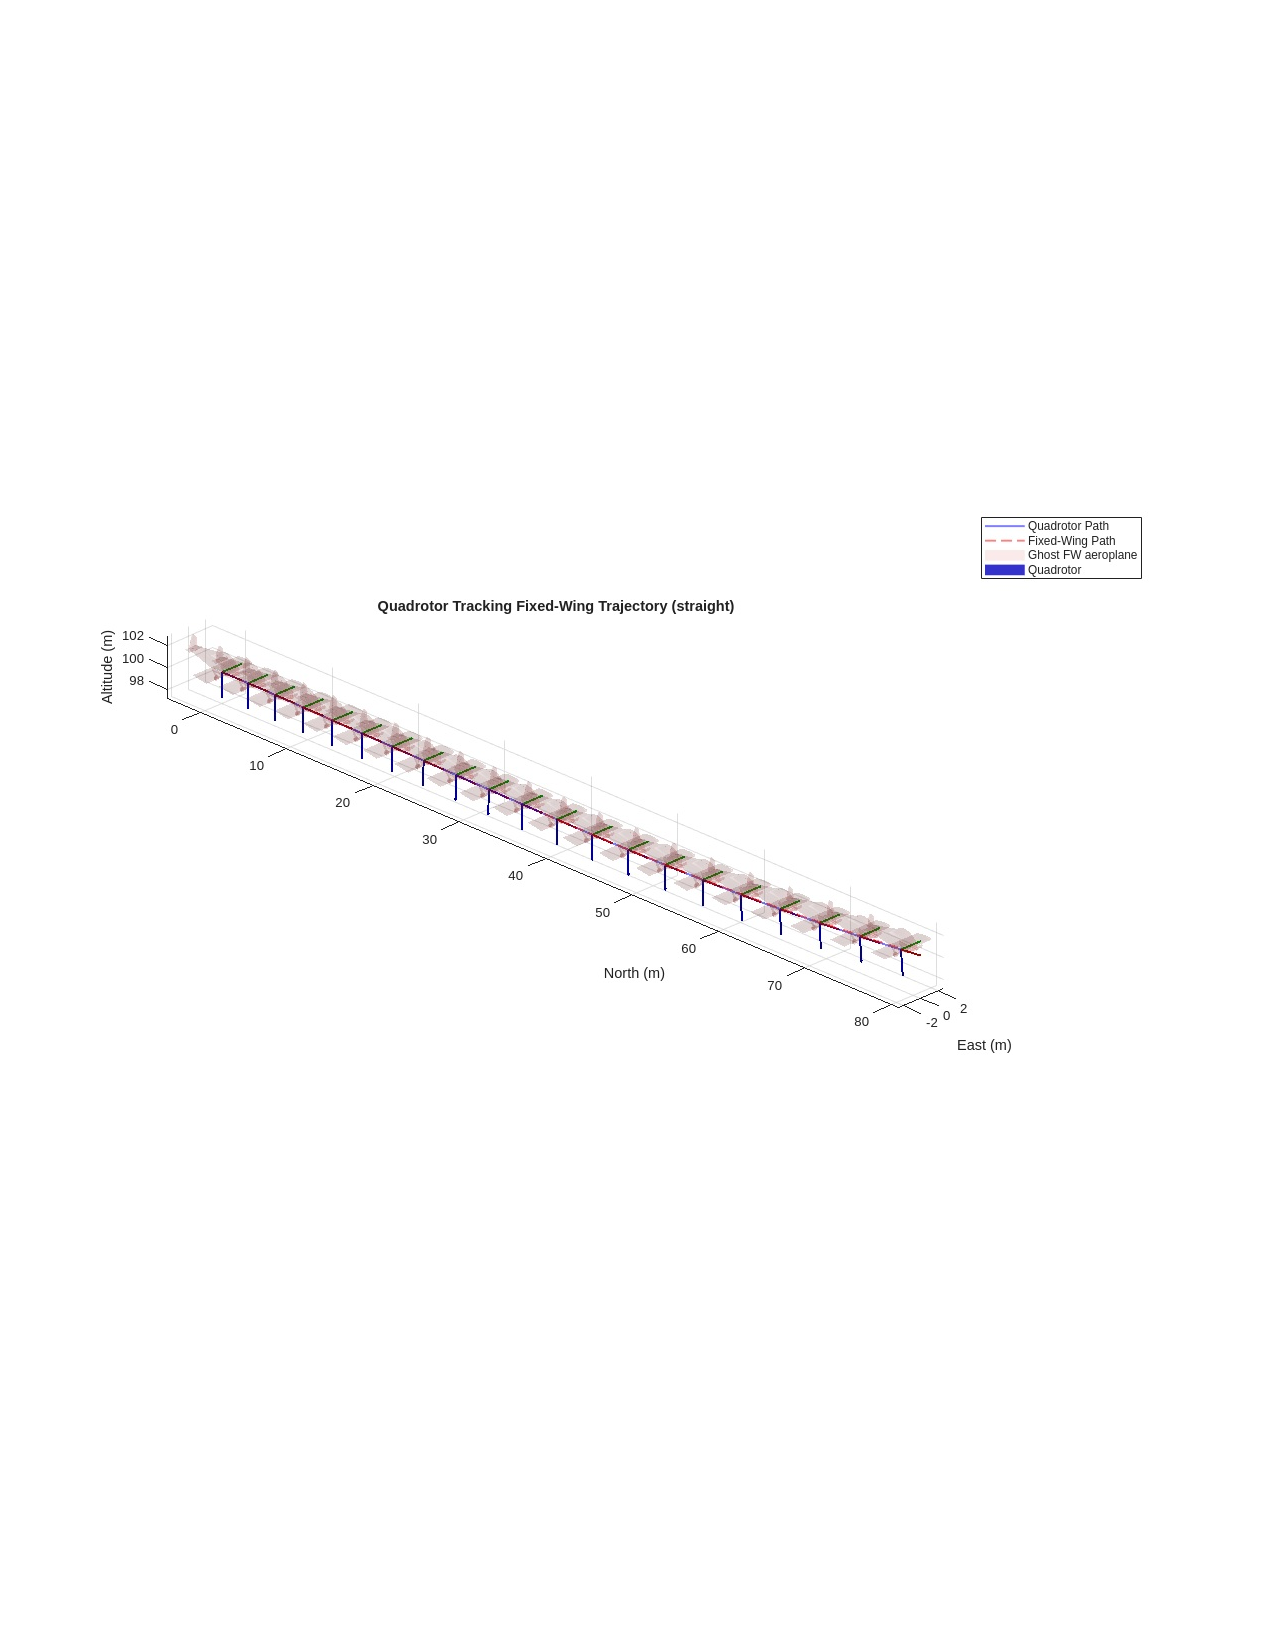
\includegraphics[width=0.8\textwidth]{results/results_straight/3d_trajectory_straight.pdf}
    \caption{3D trajectory tracking for the straight level flight.}
    \label{fig:straight_3d_traj}
\end{figure}

\begin{figure}[h!]
    \centering
    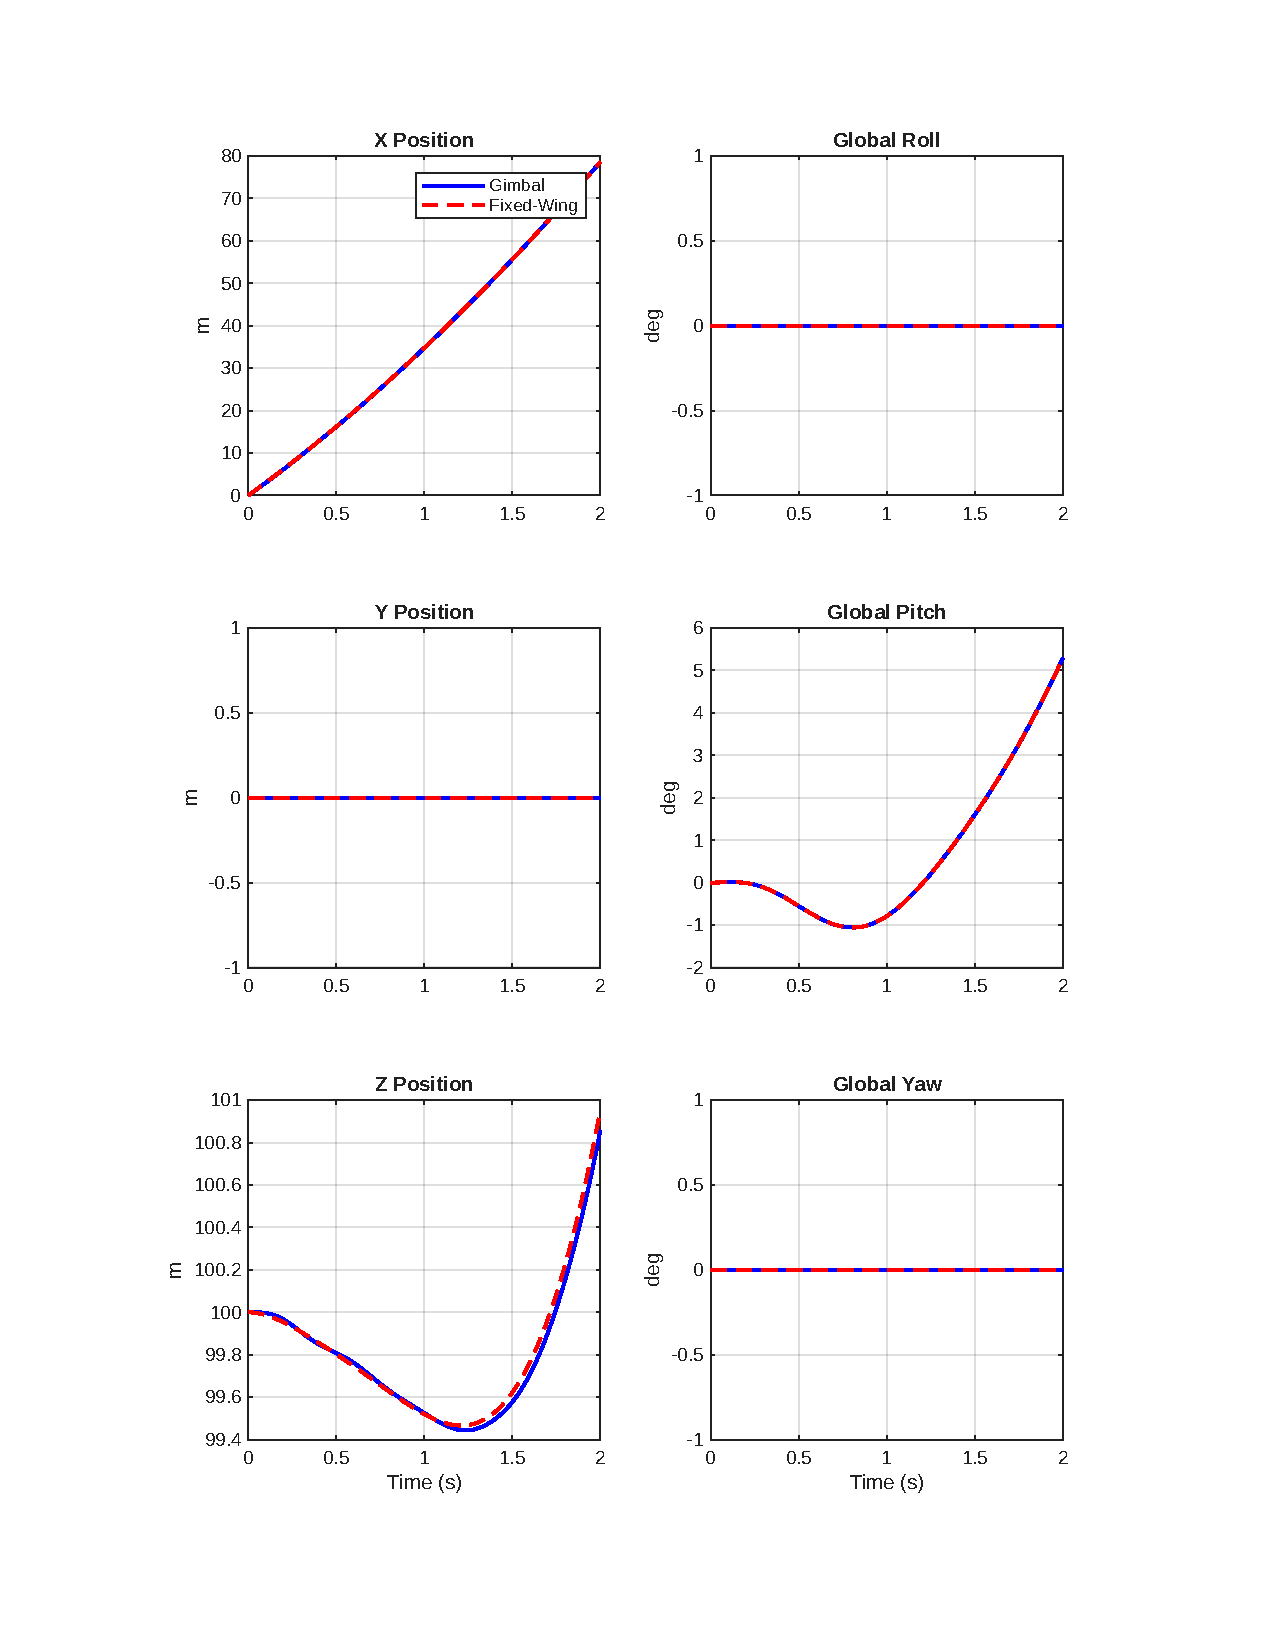
\includegraphics[width=\textwidth]{results/results_straight/position_and_orientation_straight.pdf}
    \caption{Position and orientation tracking for the straight level flight.}
    \label{fig:straight_pos_orient}
\end{figure}

\clearpage

\subsection{Trajectory 2: Loop}
To test the limits of the proposed DFL controller, a more complex flight maneuver in the form of a loop is executed. The fixed-wing aircraft performs this by applying a constant elevator input of -0.25 rad. The results show that the drone accurately follows this challenging trajectory. The gimbal compensates for the drone's movements, ensuring that the tracking direction accurately follows the fixed-wing's front-facing direction, as shown in the figures.

\begin{figure}[h!]
    \centering
    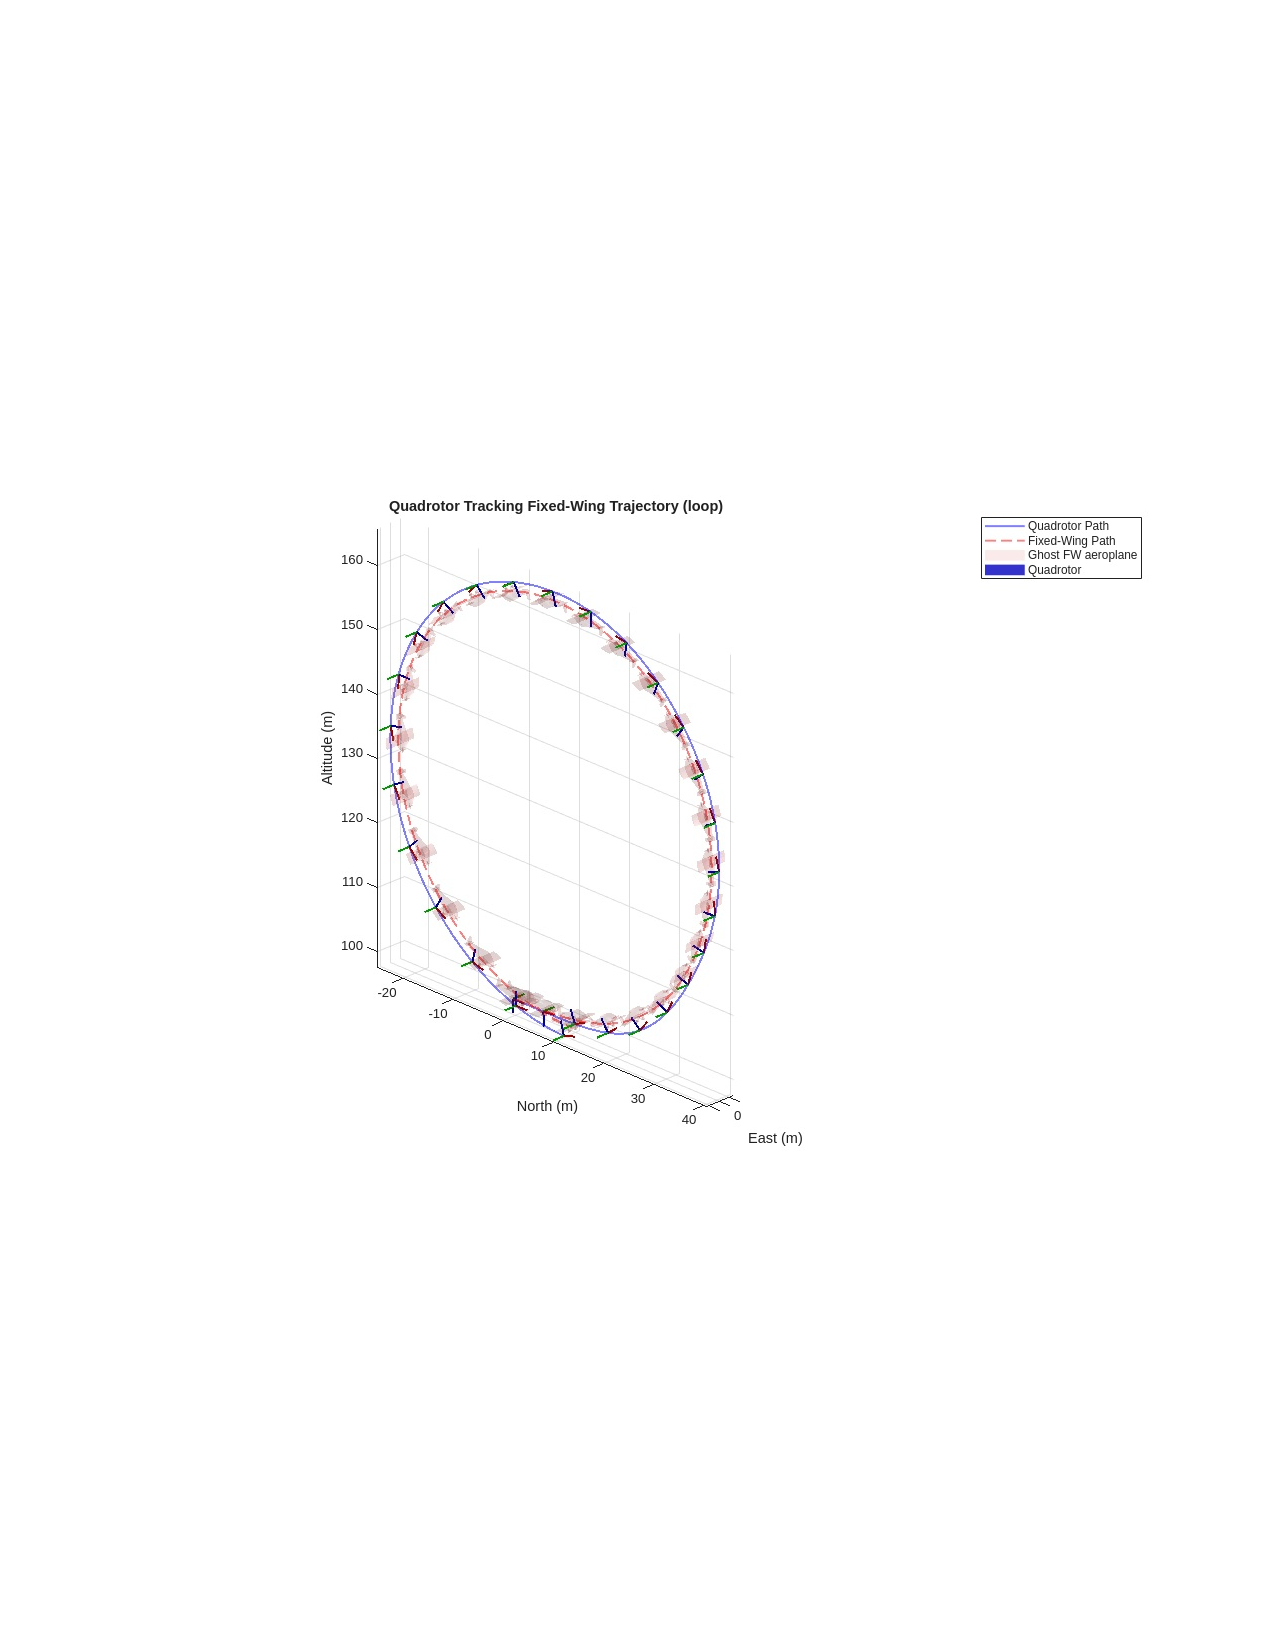
\includegraphics[width=0.8\textwidth]{results/results_loop/3d_trajectory_loop.pdf}
    \caption{3D trajectory tracking for the loop maneuver.}
    \label{fig:loop_3d_traj}
\end{figure}

\begin{figure}[h!]
    \centering
    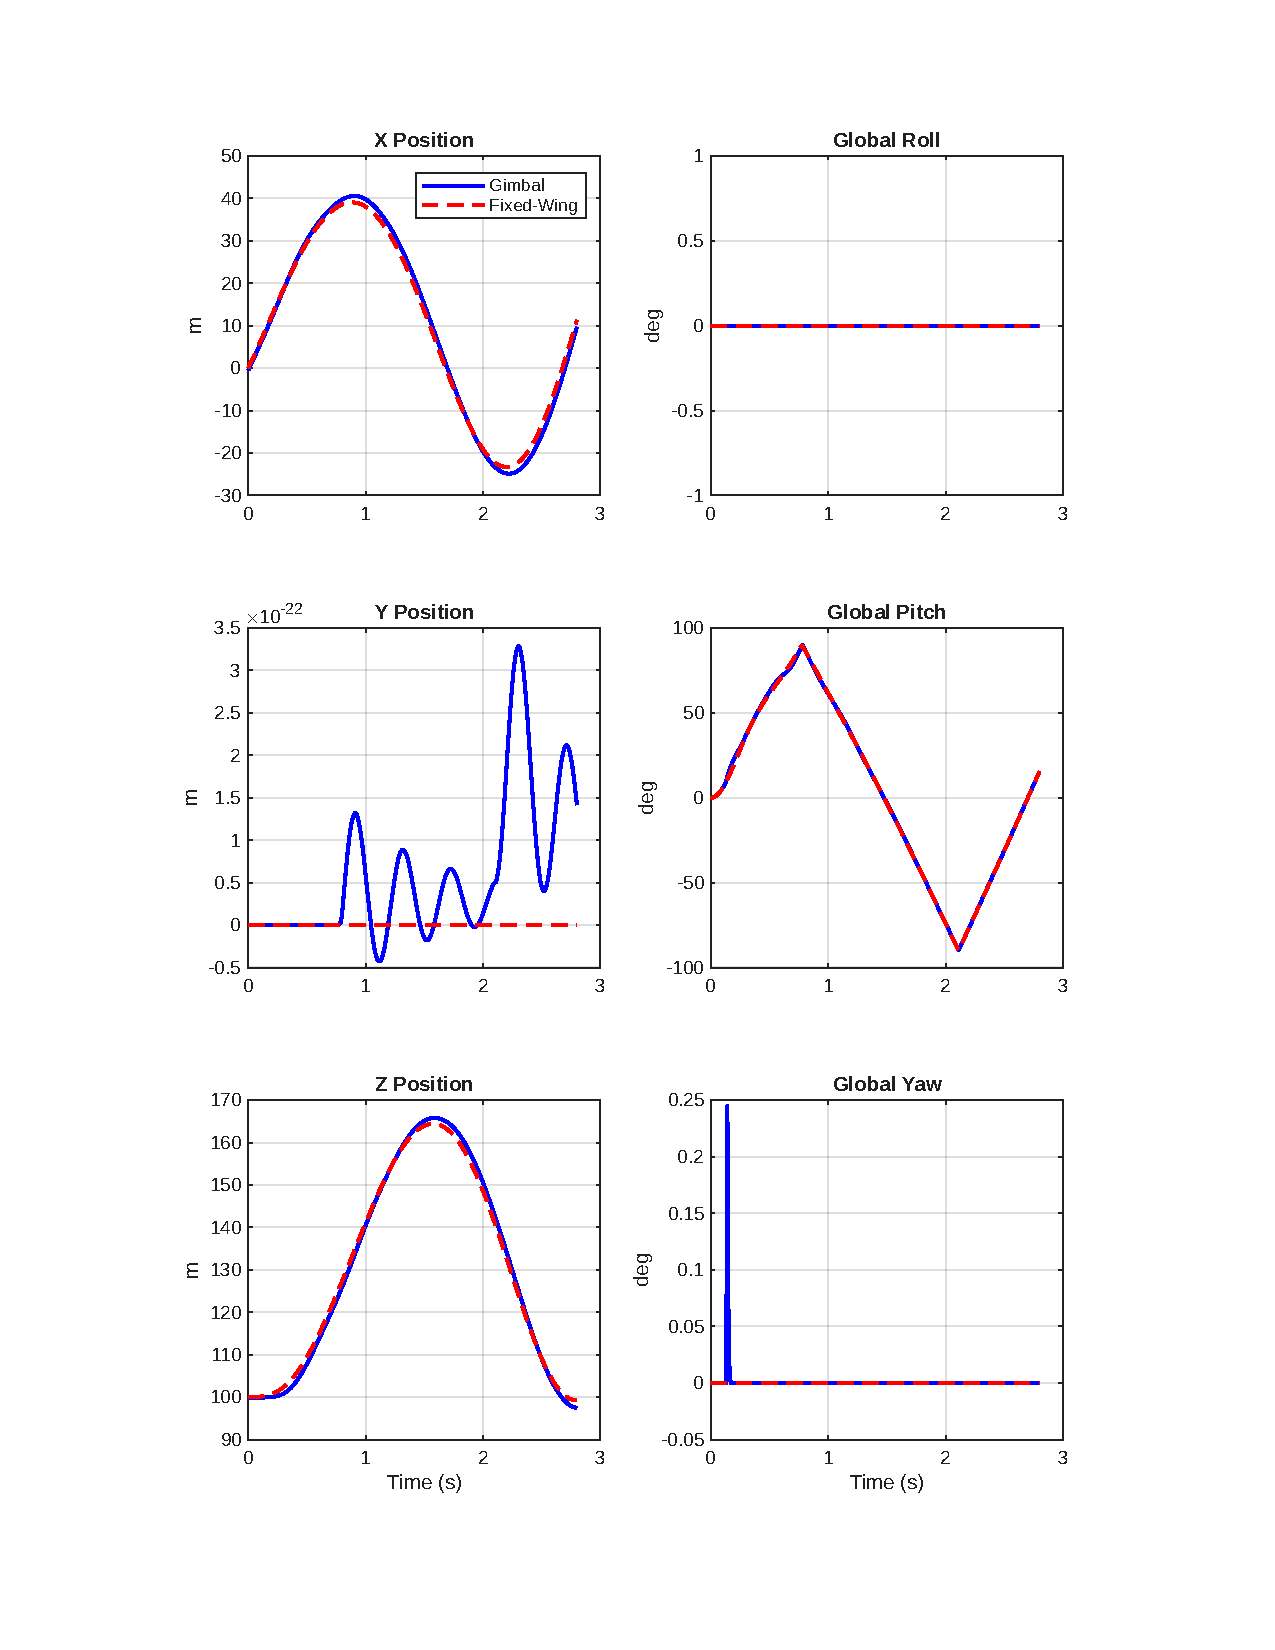
\includegraphics[width=\textwidth]{results/results_loop/position_and_orientation_loop.pdf}
    \caption{Position and orientation tracking for the loop maneuver.}
    \label{fig:loop_pos_orient}
\end{figure}

\begin{figure}[h!]
    \centering
    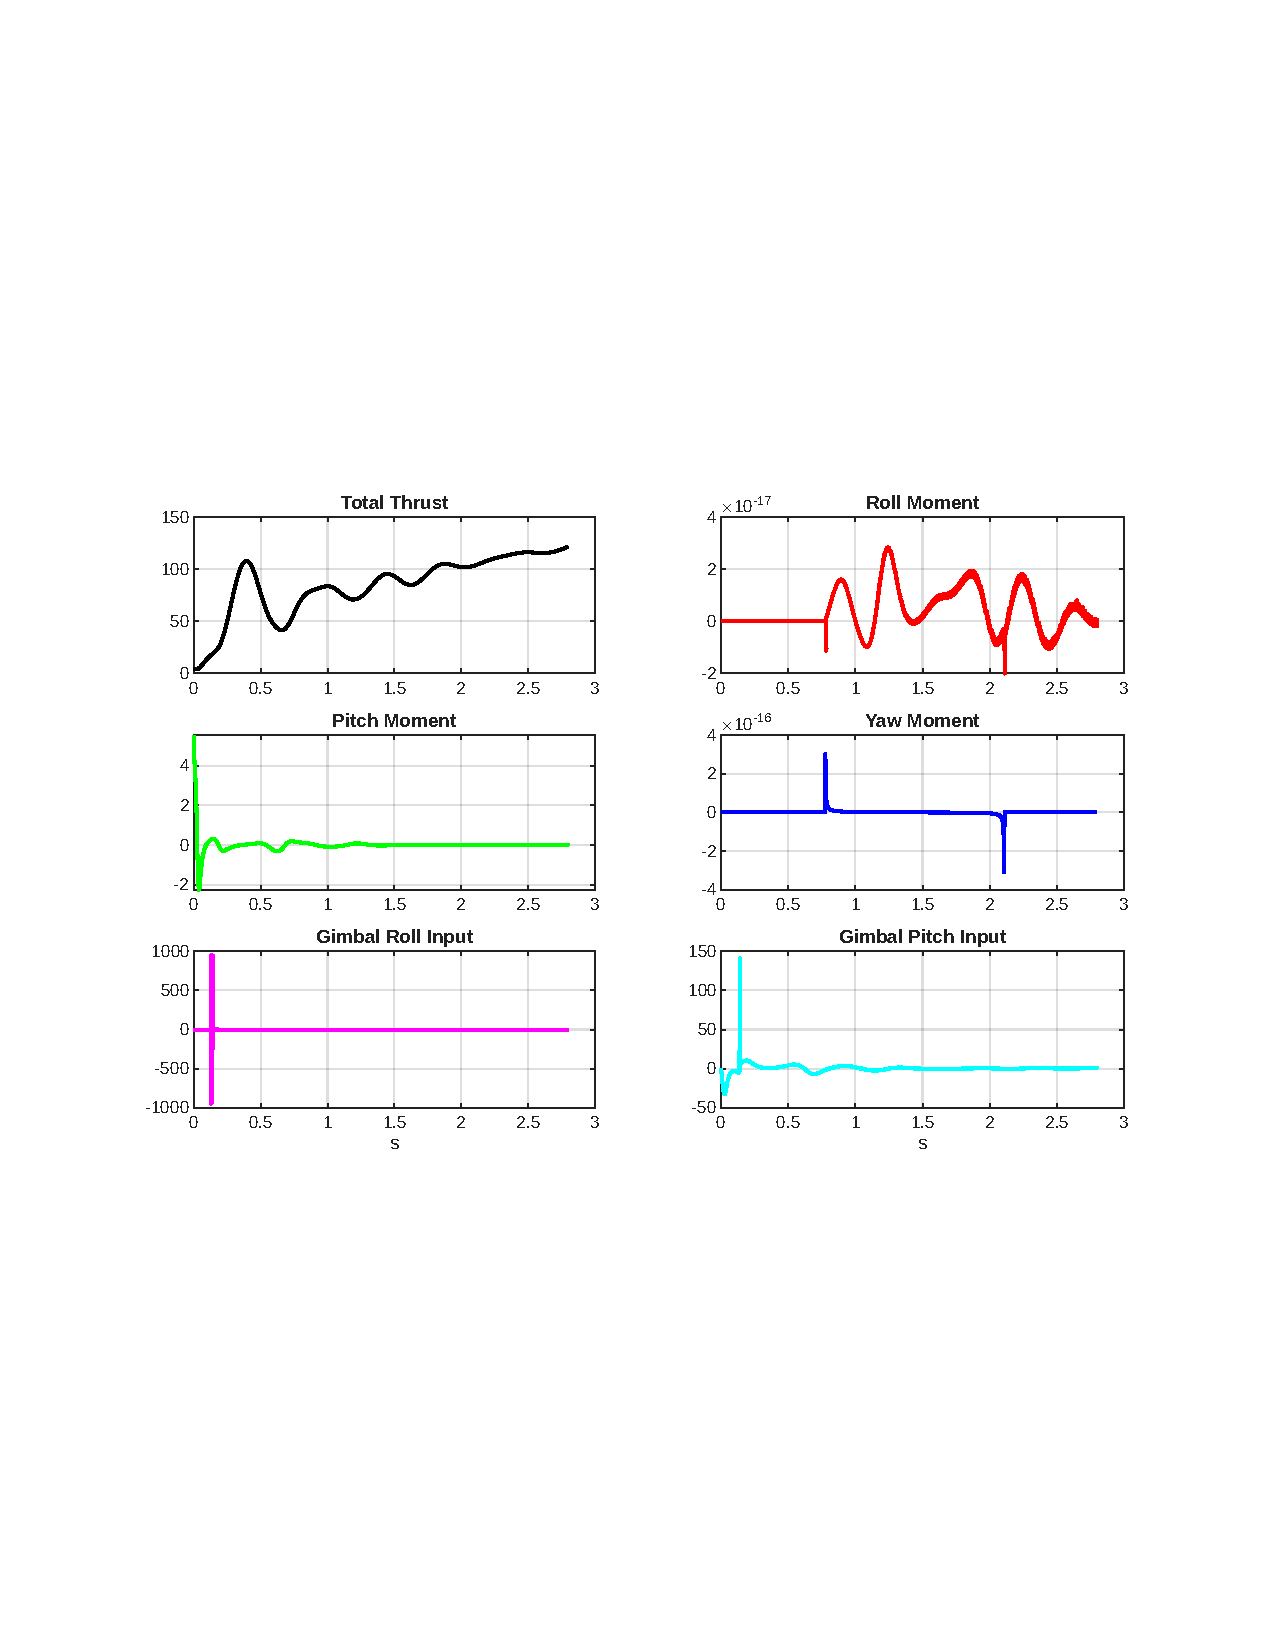
\includegraphics[width=\textwidth]{results/results_loop/control_inputs_loop.pdf}
    \caption{Control inputs for the loop maneuver.}
    \label{fig:loop_control}
\end{figure}

\end{document}
